\documentclass[english,10pt,a4paper]{article}
\usepackage[utf8]{inputenc}
\usepackage[T1]{fontenc}
\usepackage{babel}
\usepackage{graphicx}
\usepackage{cancel}
\usepackage{tikz}
\usepackage{pgfplots}
\pgfplotsset{compat=1.15}
\usepackage{mathrsfs}
\usetikzlibrary{arrows}
\usetikzlibrary{arrows,positioning,shapes,fit,calc}

\pgfdeclarelayer{background}
\pgfsetlayers{background,main}

\title{Apuntes }
\author{Samuel Ortiz}
\begin{document}
	\begin{titlepage}
		\centering
		{
\includegraphics[width=0.2\textwidth]{logo}\par}
		\vspace{1cm}
		{\bfseries\LARGE Universidad Autonoma Del Estado De Mexico\par}
		\vspace{1cm}
		{\scshape\Large Unidad Academica Profesional Tianguistenco \par}
		\vspace{3cm}
		{\scshape\Huge Apuntes de semestre\par}
		\vspace{3cm}
		{\itshape\Large Proyecto Fin de semestre \par}
		\vfill
		{\Large Autores: \par}
		{\Large Samuel Ortiz \& Axel Rebollo \& Alonso Bernal \& Eduardo De Rosas\par}
		\vfill
		{\Large Mayo 2023 \par}
		\end{titlepage}
		\newpage
		
		
	\begin{titlepage}
		\centering 
%				{\bfseries\LARGE  Temario \par}
				\tableofcontents

\end{titlepage}
\newpage
\section{Funciones I}
	\subsection{Tipos de Funciones y su representacion}
		\subsubsection{Dominio,codominio rango}
			Definicion de funcion $F$ en un conjunto $D$, llamado dominio a otro conjunto $Y$ llamado codominio (rango) es una regla que asigna a acada elemento  $X \exists D$ un unico elemento $f(x)  fy$
			 \vspace{0.3cm} \\
			 
			
			Funcion: 
			es una relacion que se cumple todo elemento del dominio tiene asignado exactamente un elemento o mas del rango \\
			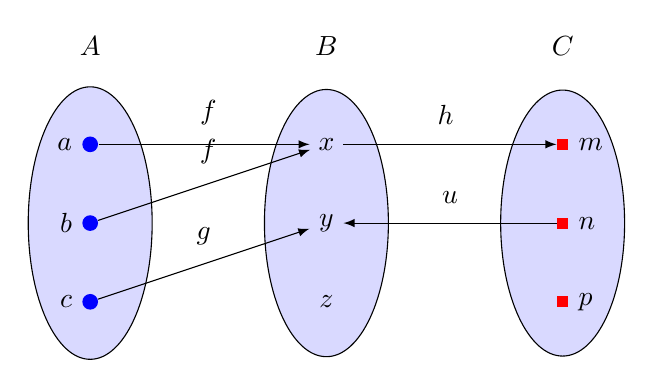
\begin{tikzpicture}[
				every node/.style={on grid},
				setA/.style={fill=blue,circle,inner sep=2pt},
				setC/.style={fill=red,rectangle,inner sep=2pt},
				every fit/.style={draw,fill=blue!15,ellipse,text width=25pt},
				>=latex
				]
				
				% set A
				\node[setA,label=left:$a$] (a) {};
				\node [setA,below = of a,label=left:$b$] (b) {};
				\node [setA,below = of b,label=left:$c$] (c) {};
				\node[above=of a,anchor=south] {$A$};
				
				% set B
				\node[inner sep=0pt,right=3cm of a] (x) {$x$};
				\node[below = of x] (y) {$y$};
				\node[inner sep=0pt,below = of y] (z) {$z$};
				\node[above=of x,anchor=south] {$B$};
				
				% set C
				\node[setC,label=right:$m$,right = 3cm of x] (m) {};
				\node[setC,label=right:$n$,below = of m] (n) {};
				\node[setC,label=right:$p$,below = of n] (p) {};
				\node[above=of m,anchor=south] {$C$};
				
				% the arrows
				\draw[->,shorten >= 3pt] (a) -- node[label=above:$f$] {} (x);
				\draw[->,shorten >= 3pt] (b) -- node[label=above:$f$] {} (x);
				\draw[->] (c) -- node[label=above:$g$] {} (y);
				\draw[->,shorten <= 3pt] (x) -- node[label=above:$h$] {} (m);
				\draw[->] (n) -- node[label=above:$u$] {} (y);
				
				% the boxes around the sets
				\begin{pgfonlayer}{background}
					\node[fit= (a)  (c) ] {};
					\node[fit= (x) (z) ] {};
					\node[fit= (m) (p)] {};
				\end{pgfonlayer}
			\end{tikzpicture}\\
			Dominio\\
			$F(x)=x+1$\\
			
			\begin{tabular}{|c|c|c|c|c|c|}
				\hline
				$X$&$-2$&$-1$&$0$&$1$ & $2$\\
				\hline
				$F(x)$&$-1$&$0$&$1$&$2$ & $3$\\		
				\hline		

			\end{tabular}\\
			$f(-2)=-2+1=-1$\\
						$f(-1)=-1+1=0$\\
									$f(0)=0+1=1$\\
												$f(2)=2+1=3$\\
												\definecolor{qqwuqq}{rgb}{0,0.39215686274509803,0}
											{	\center\begin{tikzpicture}[scale=0.5]
													\begin{axis}[
														x=1cm,y=1cm,
														axis lines=middle,
%														ymajorgrids=true,
%														xmajorgrids=true,
														xmin=-5.34054317034895,
														xmax=5.110698393729274,
														ymin=-5.791078623478701,
														ymax=5.070573901112545,
														xtick={-11,-10,...,15},
														ytick={-4,-3,...,7},]
														\clip(-11.34054317034895,-4.791078623478701) rectangle (15.110698393729274,7.070573901112545);
														\draw[line width=2pt,color=qqwuqq,smooth,samples=100,domain=-11.34054317034895:15.110698393729274] plot(\x,{(\x)+1});
														\begin{scriptsize}
															\draw[color=qqwuqq] (-5.641104380298946,-4.54142371921369) node {$F$};
														\end{scriptsize}
													\end{axis}
												\end{tikzpicture}\\
												
											}
												\newpage
									
$F(x)=2x$\\

	
\begin{tabular}{|c|c|c|c|c|c|c|}
	\hline
	$x$&$-3$&$-2$&$-1$&$0$&$1$ & $2$\\
	\hline
	$F(x)$&$-6$&$-4$&$-2$&$0$ & $2$&$4$\\		
	\hline		
	
\end{tabular}\\
$f(-3)=2(-3)=-3$\\
$f(-2)=2(-2)=-4$\\
$f(-1)=2(-1)=-2$\\
$f(0)=2(0)=-0$\\
$f(1)=2(1)=2$\\
$f(2)=2(2)=4$\\



{\definecolor{ccqqqq}{rgb}{0.8,0,0}
	\center\begin{tikzpicture}[scale=0.5]
		\begin{axis}[
			x=1cm,y=1cm,
			axis lines=middle,
			%		ymajorgrids=true,
			%		xmajorgrids=true,
			xmin=-5.34054317034895,
			xmax=5.110698393729274,
			ymin=-5.113803255821277,
			ymax=5.39329853345512,
			xtick={-11,-10,...,15},
			ytick={-5,-4,...,7},]
			\clip(-11.34054317034895,-5.113803255821277) rectangle (15.110698393729274,7.39329853345512);
			\draw[line width=2pt,color=ccqqqq,smooth,samples=100,domain=-11.34054317034895:15.110698393729274] plot(\x,{2*(\x)});
			\begin{scriptsize}
				\draw[color=ccqqqq] (-2.4503929209119772,-4.851970063543338) node {$f$};
			\end{scriptsize}
		\end{axis}
\end{tikzpicture}\\
}
$F(x)=-4x+2y=6$\\

\begin{tabular}{|c|c|c|c|}
	\hline
	$x$&$0$&$1$&$2$\\
	\hline
		$f(x)$&$3$&$5$&$7$\\
		\hline
\end{tabular}\\

$f(0)=-4(0)+2y=6$\\
$y=3$
$f(1)=-4(1)+2y=6$\\
$y=5$
$f(2)=-4(2)+2y=6$\\
$y=7$\\

{
\definecolor{ududff}{rgb}{0.30196078431372547,0.30196078431372547,1}
\definecolor{xdxdff}{rgb}{0.49019607843137253,0.49019607843137253,1}
\center\begin{tikzpicture}[scale=0.5]
	\begin{axis}[
		x=1cm,y=1cm,
		axis lines=middle,
%		ymajorgrids=true,
%		xmajorgrids=true,
		xmin=-5.329660772758457,
		xmax=5.8764363248802,
		ymin=-5.69499790003358,
		ymax=5.117171605177036,
		xtick={-9,-8,...,12},
		ytick={-5,-4,...,8},]
		\clip(-9.329660772758457,-4.69499790003358) rectangle (12.8764363248802,8.117171605177036);
		\draw [line width=2pt] (0,3)-- (1,5);
		\draw [line width=2pt] (2,7)-- (1,5);
		\begin{scriptsize}
			\draw [fill=xdxdff] (0,3) circle (2.5pt);
			\draw[color=xdxdff] (0.1016928260139165,3.2705037835856783) node {$A$};
			\draw [fill=ududff] (1,5) circle (2.5pt);
			\draw[color=ududff] (1.0997196618628446,5.266557455283534) node {$B$};
			\draw [fill=ududff] (2,7) circle (2.5pt);
			\draw[color=ududff] (2.0977464977117735,7.26261112698139) node {$C$};
			\draw[color=black] (0.7254595984194967,4.056449916816709) node {$f$};
			\draw[color=black] (1.3617017062731884,6.23963362023624) node {$g$};
		\end{scriptsize}
	\end{axis}
\end{tikzpicture}\\

}
\newpage
$f(x)=-2y=-8$\\


\begin{tabular}{|c|c|c|c|}
	\hline
	$x$&$0$&$1$&$2$\\
	\hline
	$f(x)$&$4$&$-1$&$-2$\\
	\hline
	

\end{tabular}\\

{{\definecolor{ududff}{rgb}{0.30196078431372547,0.30196078431372547,1}
	\definecolor{xdxdff}{rgb}{0.49019607843137253,0.49019607843137253,1}
	\center\begin{tikzpicture}[scale=0.5]
		\begin{axis}[
			x=1cm,y=1cm,
			axis lines=middle,
%			ymajorgrids=true,
%			xmajorgrids=true,
			xmin=-5.72,
			xmax=5.72,
			ymin=-5.74,
			ymax=5.74,
			xtick={-21,-20,...,21},
			ytick={-9,-8,...,9},]
			\clip(-21.72,-9.74) rectangle (21.72,9.74);
			\draw [line width=2pt] (-2,2)-- (1,1);
			\draw [line width=2pt] (4,0)-- (1,1);
			\begin{scriptsize}
				\draw [fill=xdxdff] (4,0) circle (2.5pt);
				\draw[color=xdxdff] (4.16,0.43) node {$A$};
				\draw [fill=ududff] (1,1) circle (2.5pt);
				\draw[color=ududff] (1.16,1.43) node {$B$};
				\draw [fill=ududff] (-2,2) circle (2.5pt);
				\draw[color=ududff] (-1.84,2.43) node {$C$};
				\draw[color=black] (-0.54,1.43) node {$f$};
				\draw[color=black] (2.68,1.05) node {$g$};
			\end{scriptsize}
		\end{axis}
	\end{tikzpicture}\\
	
}
$f(x)=x^2$\\
\begin{tabular}{|c|c|c|c|c|c|c|c|c|}
	\hline
	$xf$&$-2$&$0$&$1$&$2$&$3$\\
	\hline
		$f(x)$&$4$&$1$&$0$&$6$&$6$\\
		\hline
	
	

\end{tabular}\\
$f(-2)=-2^{2}=4$\\
$f(-1)=-1^{2}=2$\\
$f(-2)=-0^{2}=0$\\
$f(1)=-1^{2}=1$\\
$f(2)=2^{2}=4$\\
$f(3)=3^{2}=4$\\
{\definecolor{qqwuqq}{rgb}{0,0.39215686274509803,0}
	\center\begin{tikzpicture}[scale=0.5]
		\begin{axis}[
			x=1cm,y=1cm,
			axis lines=middle,
			xmin=-5.72,
			xmax=5.72,
			ymin=-5.27,
			ymax=5.27,
			xtick={-5,-4,...,5},
			ytick={-5,-4,...,5},
			]
			\clip(-5.72,-10.27) rectangle (5.72,10.27);
			\draw[line width=2pt,color=qqwuqq,smooth,samples=100,domain=-5.72:5.72] plot(\x,{(\x)^(2)});
			\begin{scriptsize}
				\draw[color=qqwuqq] (-3.1,10.02) node {$f$};
			\end{scriptsize}
		\end{axis}
	\end{tikzpicture}\\
	

}
\newpage
\subsection{Operaciones de funciones }
\subsubsection{Operaciones fundamentales}
\subsubsection{Composición de funciones.}
Las operacioens de suma,resta.multiplicacion y division entre funciones son posibles y semejantes a las correspondientes efectados con los numeros\\
Definicion:\\
son $f$ y $g$ dos funciones y supongamos que $Df$ y $Dg$ denotan los dominios de $f$ y $g$ respectivamente .La funcion  $f$ y $g$ estan definidas por \\
\begin{enumerate}
	\item $(f+g)(x)$
		\item $(f-g)(x)$
			\item $(g+f)(x)$
				\item $(f\cdot g)(x)$
							\item $(g/ f)(x)$
								\item $(f/g)(x)$
							
							
	

\end{enumerate} 
\begin{enumerate}
\item {\center $f(x)=4x+3$\\
	$g(x)=3x-7$\\
	$f+g(x)=f(x)+g(x)$\\
	$=4x+3+3x-7$\\
	$7x-4$\\
	
	
}		
\item{ \center$f-g(x)$\\
	$=4x+3-(3x-7)$\\
	$=4x+3-3x+7$\\
	$x+10$\\
	
	}	
	\item { \center$(g-f)(x)=g-f(x)=g(x)-f(x)$\\
		$3x-7-(4x+3)$\\
		$-x-10$\\
		
	}				
	\item {\center $(f\cdot g)(x)$\\
				$(3x-7)\cdot (4x+3)$\\
				$12x^{2}-28-9x-21$\\
				$12x^{2}-19x-21$\\
	}
	
	
	\item   {\center $\frac{g}{g}(x)=\frac{f(x)}{g(x)}=g(x)\neq 0$\\
		$=\frac{4x+3}{3x-7}$\\
		

	}
	\item {\center $\frac{g}{f}(x)=\frac{g(x)}{f(x)}=\frac{3x-7}{4x+3}$\\
	}

\end{enumerate}
\newpage
{\centering\emph{Ejercicios}\\
}


\begin{enumerate}
	\item {\center $f(x)=x-3$\\
	}
	\item{\center$g(x)=x^{2}+x-12$\\
		
	
	
	
	}
\end{enumerate}


\begin{enumerate}
\item {$(f+g)(x)=x-3+x^{2}+x-12$\\
	$x^{2}+2x-15$\\
	
	
	
	
	}
	\item {$(f-g)(x)=(x-3)-(x^{2}+x-12)$\\
		$x-3-x^{2}-x+12$\\
		$=-x^{2}+9$\\
	}
\item	{$(g-f)(x)=x^{2}+x-12-(x-3)$\\
	$x^{2}+x-12-x+3$\\
	
	$x^2+x-12-x+3$\\
	$x^{x}-9$

}
\item {$(g\cdot f)(x)=(x-3)(x^{2}+x-12)$\\
	$x^{3}+x^{2}-12x$\\
			$-3x^{2}-3x+36$\\
			$=x^{3}-2x^{2}-15x+36$



}
\item {$(\frac{f}{g})(x)=\frac{x-3}{x^{2}+x-12}=$\\
	$\frac{x-3}{(x-3)(x+4)}$\\
	=$\frac{1}{x+4}$\\
	
	
	
}
\item {$(\frac{g}{f})(x)=\frac{x^{2}+x-12}{x-3}=$\\
	$\frac{\cancel{(x-3)}(x-4)}{\cancel{(x-3)}}$
	



}
	
\end{enumerate}
\newpage
{\centering\emph{Ejercicios}\\
}

\begin{enumerate}
	
	
\item {\center $f(x)=2x+4$\\
	}
	\item {\center$f(g)=x-10$\\
	}

\end{enumerate}

\begin{enumerate}
\item{$(f-g)(x)=2x+4-(x-10)$\\
	$2x+4-x+10$\\
	$x+14$
	
}
\item {$(g-f)(x)=x-10-1(2x+4)$\\
	$x-10-2x+4$\\
	$-x-14$\\
	
	
	
}
\item {$(f+g)(x)=2x+4+x+10=3x-6$\\
}
\item {$(\frac{f}{g})(x)=\frac{f(x)}{g(x)}=$\\
	$\frac{2x+4}{x-10}$\\

}
\item {$(\frac{g}{f})(x)=\frac{g(x)}{f(x)}=$\\
	$\frac{x-10}{2x+4}$\\
}

\item {$f\cdot g (x)=f(x)\cdot g(x)=$\\
		$=(2x+4)(x-10)=$\\
		$2x^{2}-20x+4-40$\\
		$2x^{2}-16-40$
		




}





\end{enumerate}
\newpage 
\section{title}
\newpage
\section{Derivadas}
\subsection{ Definición de la derivada.}
\emph{Derivada}\\
Derivada es una función de una variable es el limite de la razón de incremento de la función la incremento de la variable independiente cuando este tiende a $0$. \\
Cuando el limite de esta razón existe , se dice que la función es desiderable o que tienen una derivada .\\
La función puede darse mediante símbolos , en la forma siguiente\\
{\center $y=f(x)$\\}
símbolos para representar la derivada puesto que $ \triangle y$ y $\triangle x$ son siempre cantidades finitas y tienen valores definidos la expresión es la siguiente.\\
{\center $\frac{\triangle y} {\triangle x}$\\}
\vspace{1cm}
{\center \emph{Formula}$=\frac{f(x+\triangle x)-f(x)}{\triangle x}$\hspace{1cm}$\triangle x\rightarrow 0$\\
}

\[
\lim_{\triangle x \to 0}{\frac{f(x+\triangle x=)-f(x)}{\triangle x}}
\]\hspace{1cm} \begin{enumerate}
\item {$f\prime(x)$}
\end{enumerate}


			
			
			
			
		


		
		
\end{document}